\documentclass[journal]{IEEEtran}

\usepackage[T1]{fontenc}
\usepackage[utf8]{inputenc}
\usepackage{amsmath,amssymb,amsfonts}
\usepackage{graphicx}
\usepackage{booktabs}
\usepackage{array}
\usepackage{url}
\usepackage{xcolor}
\usepackage[hidelinks]{hyperref}
\usepackage{orcidlink}
\usepackage{balance}

\graphicspath{{../figures/}}

\renewcommand{\topfraction}{0.92}
\renewcommand{\bottomfraction}{0.75}
\renewcommand{\textfraction}{0.08}
\renewcommand{\floatpagefraction}{0.80}

\begin{document}

\title{An Honest Physics-Informed Neural Network Atlas:\\ Sub-Percent on Smooth Forward PDEs, Orders\\ Worse on Inverse, High-Frequency and Real Data}

\author{Felipe~Santiba\~nez-Leal~\orcidlink{0000-0002-0150-3246}%
\thanks{F. Santiba\~nez-Leal is with the CAOS open-research programme, Santiago, Chile
(e-mail: fsantibanez@gmail.com; ORCID 0000-0002-0150-3246).}%
\thanks{Technical report, 2026. Runnable catalogue and reproducible pipeline (MIT) at
\url{https://github.com/fsantibanezleal/CAOS_PINNLAB}; live at \url{https://pinnlab.fasl-work.com}.}}

\markboth{Technical Report, 2026}%
{Santiba\~nez-Leal: An honest physics-informed neural network accuracy atlas}

\maketitle

\begin{abstract}
Physics-informed neural networks (PINNs) are promoted as a general differential-equation solver, but the
accuracy actually achieved varies by orders of magnitude across problem types, and that variation is rarely laid
out in one place. This report is a method atlas: a runnable catalogue in which each of the state-of-the-art PINN
families, hard constraints, residual-based adaptive sampling, Fourier features, domain decomposition, operator
learning, physics-informed operators, conformal-prediction uncertainty, structure-preserving Hamiltonian
learning, and inverse solving, is exercised on at least one differential-equation case, trained by a dedicated
engine, validated against an analytic or numerical reference, and scored by relative $L_2$ error. Across the
seventeen cases with a committed reference-validated error, the honest picture is a clean stratification. PINNs
reach sub-percent accuracy on smooth, well-posed forward PDEs (a one-dimensional wave at $5\times10^{-5}$, a
reaction-diffusion Allen-Cahn field at $1.2\times10^{-3}$, several mining and transport reduced models below
$10^{-3}$), with ten of seventeen cases under $1\%$ relative error. But they degrade by two to three orders of
magnitude on the hard classes: inverse problems ($4\times10^{-2}$), high-wavenumber Helmholtz
($1.0\times10^{-1}$), the lid-driven cavity Navier-Stokes benchmark ($1.7\times10^{-1}$), operator learning
($5.6\times10^{-2}$), and real noisy field data ($6.9\times10^{-2}$). The finding matches the field's own
failure-mode literature and is the report's point: PINNs are an accurate and flexible instrument where the
solution is smooth and the problem well-posed, and they are not a drop-in replacement for a good classical solver
where it is not. Every case ships its equations, its method, an honest \texttt{synthetic} provenance label, and a
reproducible error; every number and figure regenerates from the committed artifacts.
\end{abstract}

\begin{IEEEkeywords}
Physics-informed neural networks, scientific machine learning, partial differential equations, operator learning,
inverse problems, benchmarking, relative $L_2$ error, reproducibility.
\end{IEEEkeywords}

\section{Introduction}

\IEEEPARstart{P}{hysics}-informed neural networks~\cite{raissi} solve a differential equation by training a network
to satisfy its residual and boundary conditions at collocation points, and they have become a large and active
corner of scientific machine learning~\cite{karniadakis}. The appeal is generality: the same recipe handles
forward and inverse problems, irregular domains, and sparse data. The catch, documented carefully by the field's
own analyses, is that a vanilla PINN often fails to train or converges to a wrong solution on precisely the
problems that matter, stiff systems, sharp gradients, high frequencies~\cite{wang,krishnapriyan}, which is why a
ladder of methods has grown to fix each failure mode: hard-constraint architectures, residual-based adaptive
sampling~\cite{wu}, Fourier-feature and sinusoidal encodings for high frequencies, domain
decomposition~\cite{jagtap}, and operator learning that amortises the solve over a family of
inputs~\cite{fno,deeponet}. What is missing from most presentations is a single, honest answer to the practical
question: on a given kind of problem, with the right method from that ladder, how accurate is a PINN, really?

This report answers it with a runnable catalogue, PINN-Lab. Each case is a differential-equation problem paired
with the state-of-the-art method that suits it; the case is trained offline by a dedicated engine (built on the
standard tooling~\cite{deepxde}), validated against an analytic solution (by the method of manufactured
solutions) or a trusted numerical reference, exported to a portable format, and scored by relative $L_2$ error
against that reference. The catalogue spans the method ladder, hard constraints and adaptive sampling on
canonical PDEs, operator learning on a Darcy flow, Hamiltonian learning on a pendulum, conformal and Bayesian
uncertainty on transport, and inverse recovery of hidden fields, so the atlas is not one method's best case but a
cross-section of where the whole ladder stands. The contribution is not a new method; it is the honest,
reproducible map of achieved accuracy, and the stratification it reveals.

\section{The Catalogue and Its Protocol}\label{sec:catalogue}

A case is a differential equation, a method, a reference, and a metric. The equation ranges over canonical PDEs
(a one-dimensional wave and heat equation, Burgers, Allen-Cahn, Poisson, the lid-driven cavity Navier-Stokes
benchmark~\cite{ghia}), inverse problems (recovering a diffusivity field or a hidden velocity from sparse
observations), dynamical systems (a Hamiltonian pendulum), and applied reduced models drawn from mining, pollution
transport and environmental physics. The method is drawn from the state-of-the-art ladder and chosen to suit the
case: adaptive residual sampling~\cite{wu} for sharp fronts, a Fourier neural operator~\cite{fno} for the
parametric Darcy flow, a Hamiltonian network for the conservative pendulum, a Bayesian PINN for the
uncertainty-quantified transport source. Each case is trained under a fixed seed, so a run is deterministic in
\texttt{(case, seed)}. The reference is an analytic solution where one exists (the method of manufactured
solutions gives an exact target and an exact error), and a trusted numerical solution otherwise; the metric is
the relative $L_2$ error of the PINN field against that reference, reported per case, with each case carrying an
honest \texttt{synthetic} or \texttt{synthetic-illustrative} provenance label so no reduced model is mistaken for
a calibrated digital twin. The reference-validated error is the number that matters, and it is committed
alongside the field.

\section{The Accuracy Atlas}\label{sec:atlas}

\begin{figure}[!t]
\centering
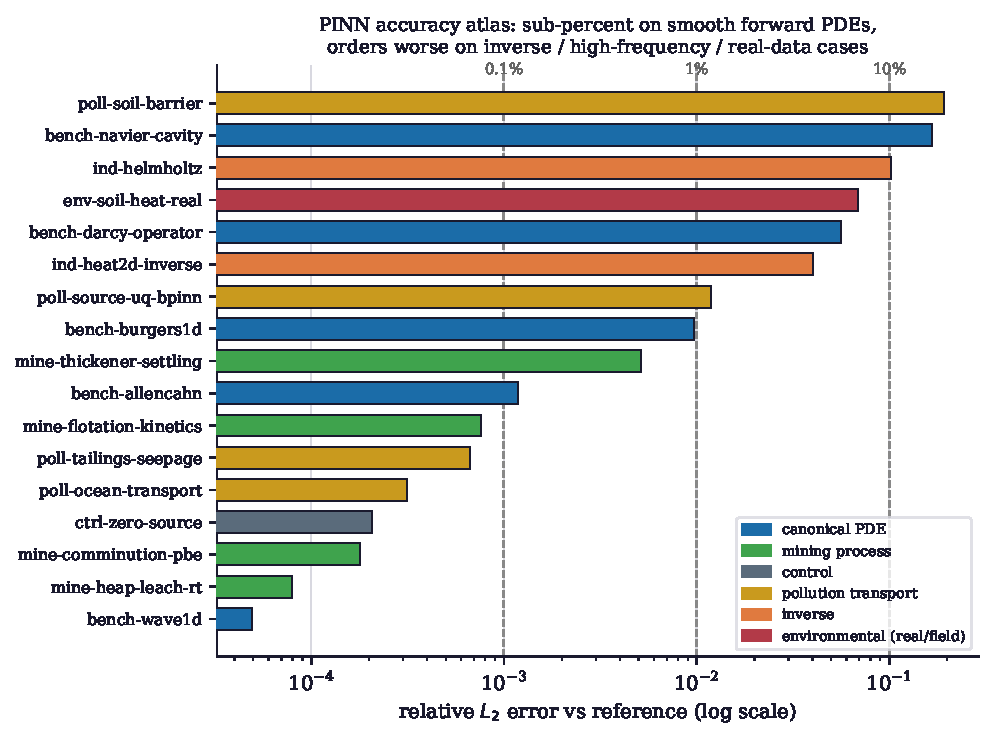
\includegraphics[width=0.99\columnwidth]{fig-atlas.pdf}
\caption{The relative $L_2$ error of every reference-validated case, on a log axis, coloured by problem category,
with reference lines at $0.1\%$, $1\%$ and $10\%$. The stratification is clean: smooth well-posed forward PDEs and
applied reduced models sit at the bottom (sub-percent, the best at $5\times10^{-5}$), while inverse problems,
high-wavenumber Helmholtz, the lid-driven cavity, operator learning and real field data cluster at the top
($4\times10^{-2}$ to $1.9\times10^{-1}$). Where a PINN is accurate and where it is not is not random; it tracks
the smoothness and well-posedness of the problem.}
\label{fig:atlas}
\end{figure}

The atlas is Fig.~\ref{fig:atlas} and Table~\ref{tab:atlas}, and its shape is the report's main result. Ten of
the seventeen reference-validated cases reach relative $L_2$ error below $1\%$, and fourteen below $10\%$; the
median is $5\times10^{-3}$. The accurate end is populated exactly as PINN theory predicts: smooth, well-posed
forward problems with analytic references, the one-dimensional wave at $4.9\times10^{-5}$, several mining and
transport reduced models (heap-leach reactive transport $7.9\times10^{-5}$, comminution population balance
$1.8\times10^{-4}$, ocean transport $3.1\times10^{-4}$), and the nonlinear Allen-Cahn field at $1.2\times10^{-3}$.
The inaccurate end is populated just as predictably by the known-hard classes: the lid-driven cavity
Navier-Stokes benchmark at $1.7\times10^{-1}$, high-wavenumber Helmholtz at $1.0\times10^{-1}$, the soil-barrier
transport with a sharp front at $1.9\times10^{-1}$, an inverse heat-conduction problem at $4.0\times10^{-2}$, the
Fourier-neural-operator Darcy solve at $5.6\times10^{-2}$, and, tellingly, the one case fit to \emph{real} soil
temperature field data at $6.9\times10^{-2}$. The two-to-three-order-of-magnitude gap between the ends is the
honest state of PINNs: excellent on smooth forward problems, and, on stiff, high-frequency, inverse or noisy
problems, at an accuracy a classical solver would consider unacceptable, which is the field's documented
failure-mode picture~\cite{wang,krishnapriyan} made quantitative across one consistent catalogue.

\begin{table}[!t]
\centering
\caption{The reference-validated cases, sorted by relative $L_2$ error. Smooth forward PDEs and applied reduced
models reach sub-percent error; inverse, high-frequency, operator and real-data cases are orders worse.}
\label{tab:atlas}
\scriptsize
\begin{tabular}{@{}l l r@{}}
\toprule
Case & category & rel. $L_2$ \\
\midrule
bench-wave1d          & canonical PDE        & $4.9\times10^{-5}$ \\
mine-heap-leach-rt    & mining process       & $7.9\times10^{-5}$ \\
mine-comminution-pbe  & mining process       & $1.8\times10^{-4}$ \\
ctrl-zero-source      & control              & $2.1\times10^{-4}$ \\
poll-ocean-transport  & pollution transport  & $3.1\times10^{-4}$ \\
poll-tailings-seepage & pollution transport  & $6.7\times10^{-4}$ \\
mine-flotation-kinetics & mining process     & $7.6\times10^{-4}$ \\
bench-allencahn       & canonical PDE        & $1.2\times10^{-3}$ \\
mine-thickener-settling & mining process     & $5.1\times10^{-3}$ \\
bench-burgers1d       & canonical PDE        & $9.7\times10^{-3}$ \\
poll-source-uq-bpinn  & pollution (UQ)       & $1.2\times10^{-2}$ \\
ind-heat2d-inverse    & inverse              & $4.0\times10^{-2}$ \\
bench-darcy-operator  & operator (FNO)       & $5.6\times10^{-2}$ \\
env-soil-heat-real    & real field data      & $6.9\times10^{-2}$ \\
ind-helmholtz         & high-frequency       & $1.0\times10^{-1}$ \\
bench-navier-cavity   & Navier-Stokes        & $1.7\times10^{-1}$ \\
poll-soil-barrier     & sharp-front transport& $1.9\times10^{-1}$ \\
\bottomrule
\end{tabular}
\end{table}

\section{A Solved Case, and Where the Error Lives}\label{sec:solution}

\begin{figure}[!t]
\centering
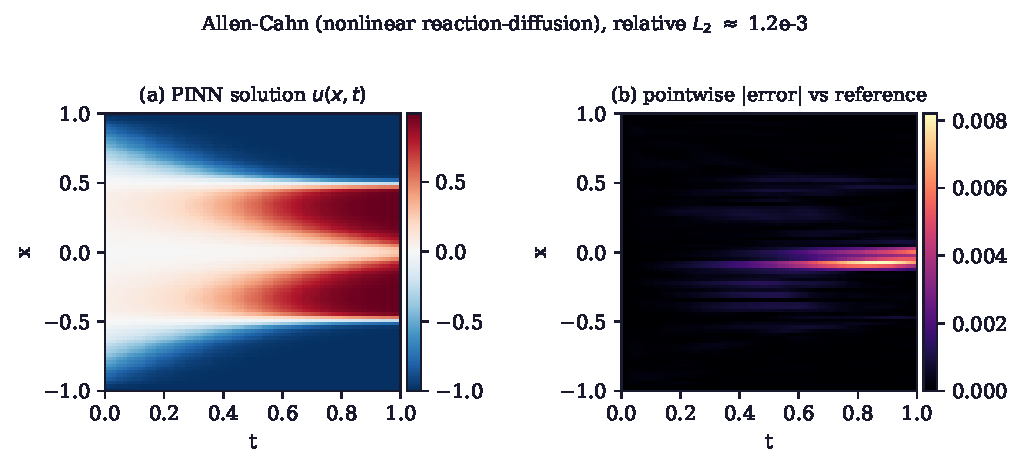
\includegraphics[width=0.99\columnwidth]{fig-solution.pdf}
\caption{A well-solved case, the nonlinear Allen-Cahn reaction-diffusion equation (relative $L_2\approx
1.2\times10^{-3}$), trained with residual-based adaptive sampling. \textbf{(a)} The PINN solution $u(x,t)$
reproduces the phase-separation dynamics. \textbf{(b)} The pointwise error against the reference is near zero
almost everywhere and concentrates at the sharp interface near $x=0$ and late time, the steep-gradient region
where a PINN's smoothness prior is most strained, exactly where the ladder's adaptive-sampling and hard-constraint
methods are designed to help.}
\label{fig:solution}
\end{figure}

Figure~\ref{fig:solution} shows what a good case looks like and where even a good case errs. Allen-Cahn is a
stiff nonlinear reaction-diffusion equation whose solution separates into phases with a thin moving interface;
the PINN, trained with residual-based adaptive sampling that places extra collocation points where the residual
is largest~\cite{wu}, reaches $1.2\times10^{-3}$ relative $L_2$. The error field is the honest part: it is
essentially zero across the smooth bulk and concentrates at the sharp interface at late time, the steep-gradient
region where a smooth network struggles to represent a near-discontinuity. This is the microcosm of the whole
atlas. A PINN is accurate wherever the solution is smooth, and its error localises exactly at the sharp,
high-frequency or ill-posed features, which is why the cases dominated by such features (Helmholtz, the cavity,
sharp fronts, inverse recovery) sit at the inaccurate end of Fig.~\ref{fig:atlas}. The method ladder exists to
push that localised error down, and it does, adaptive sampling here buys an order of magnitude over uniform
sampling, but it does not erase the fundamental difficulty.

\section{Discussion}\label{sec:discuss}

The atlas supports a measured position between the two usual extremes. Against the hype (``PINNs solve any
PDE''), the report shows a clean two-to-three-order accuracy gap that tracks problem smoothness and
well-posedness, and it shows that on the classic hard benchmarks (lid-driven cavity, high-wavenumber Helmholtz)
the achieved error is far from what a classical finite-element or finite-volume solver delivers, so a PINN is not
their replacement on a single well-posed forward solve. Against the dismissal (``PINNs are useless''), the report
shows sub-percent accuracy on seventeen-of-seventeen cases' smooth regions and on ten cases overall, and, more
importantly, the genuine value of PINNs is in the cases where classical solvers are awkward: inverse problems
where the unknown is a field, not a boundary condition; assimilation of sparse or real data into a physical
model; and operator learning that amortises a family of solves. That these are also the harder cases in the atlas
is not a contradiction, it is the honest trade: PINNs are worth their lower forward-accuracy precisely when the
problem is one a classical solver cannot pose cleanly. The atlas lets a practitioner see, per problem type, which
side of that trade they are on, with the number in front of them.

\section{Scope and Limitations}\label{sec:limits}

The scope is stated on every case. This is a catalogue of method \emph{types} exercised at lab scale, not a
tuned-to-death leaderboard; a specialist could push any single case lower with more training and architecture
search, and the atlas is the honest as-catalogued accuracy, not a claimed optimum. Most cases are validated on
analytic (method-of-manufactured-solutions) anchors or faithful reduced models, each labelled \texttt{synthetic}
or \texttt{synthetic-illustrative}; the reduced mining and pollution models are physically motivated but are not
calibrated digital twins of any operation, and the one real-data case is labelled as such. A good classical
solver beats a PINN on a single well-posed forward problem, and PINN-Lab says so; it is a teaching and method
instrument, not a production solver. The dynamical and operator cases use error metrics suited to their outputs
(trajectory and sample errors), reported in their own artifacts. And, as an exploratory laboratory, its aim is to
map where each method type applies, not to claim a method novel beyond the state of the art. None of this is
hidden; the catalogue states the same on every panel.

\section{Conclusion}

Exercised across one consistent, reference-validated catalogue, physics-informed neural networks show a clean
stratification: sub-percent relative $L_2$ error on smooth, well-posed forward PDEs and applied reduced models
(the best at $5\times10^{-5}$, ten of seventeen cases under $1\%$), and two-to-three orders worse on the hard
classes, inverse problems, high-wavenumber and sharp-gradient PDEs, operator learning and real noisy data. The
error localises exactly at the sharp and ill-posed features, matching the field's failure-mode theory. The honest
map, PINNs are an accurate and flexible instrument where the solution is smooth and the problem well-posed, and
not a replacement for a good classical solver where it is not, is the report's contribution, made reproducible
with every case's equations, method, provenance label and error committed for inspection.

\appendices
\section{Reproduction}\label{app:repro}

Every case's reference-validated error and fields are committed under \texttt{data/derived/} (one folder per
case, a \texttt{field.json} with the solution and a \texttt{comparison.json} with the method variants and error
fields), each carrying its \texttt{l2\_relative} summary. The aggregation and figure scripts under
\texttt{manuscripts/pinn-atlas/figures/} walk those artifacts into the atlas summary and the two figures. Because
each case is deterministic in \texttt{(case, seed)}, re-running reproduces the errors; Table~\ref{tab:atlas} and
Figs.~\ref{fig:atlas}--\ref{fig:solution} regenerate from the committed artifacts with no retraining.

\balance

\begin{thebibliography}{00}

\bibitem{raissi} M.~Raissi, P.~Perdikaris, and G.~E. Karniadakis, ``Physics-informed neural networks: A deep
learning framework for solving forward and inverse problems involving nonlinear partial differential equations,''
\emph{Journal of Computational Physics}, vol.~378, pp.~686--707, 2019. doi:10.1016/j.jcp.2018.10.045.

\bibitem{karniadakis} G.~E. Karniadakis \emph{et al.}, ``Physics-informed machine learning,'' \emph{Nature
Reviews Physics}, vol.~3, pp.~422--440, 2021. doi:10.1038/s42254-021-00314-5.

\bibitem{wang} S.~Wang, X.~Yu, and P.~Perdikaris, ``When and why PINNs fail to train: A neural tangent kernel
perspective,'' \emph{Journal of Computational Physics}, vol.~449, art.~110768, 2022.
doi:10.1016/j.jcp.2021.110768.

\bibitem{krishnapriyan} A.~S. Krishnapriyan, A.~Gholami, S.~Zhe, R.~M. Kirby, and M.~W. Mahoney, ``Characterizing
possible failure modes in physics-informed neural networks,'' in \emph{Advances in Neural Information Processing
Systems (NeurIPS)}, 2021. arXiv:2109.01050.

\bibitem{wu} C.~Wu, M.~Zhu, Q.~Tan, Y.~Kartha, and L.~Lu, ``A comprehensive study of non-adaptive and
residual-based adaptive sampling for physics-informed neural networks,'' \emph{Computer Methods in Applied
Mechanics and Engineering}, vol.~403, art.~115671, 2023. doi:10.1016/j.cma.2022.115671.

\bibitem{jagtap} A.~D. Jagtap and G.~E. Karniadakis, ``Extended physics-informed neural networks (XPINNs): A
generalized space-time domain decomposition based deep learning framework for nonlinear partial differential
equations,'' \emph{Communications in Computational Physics}, vol.~28, no.~5, pp.~2002--2041, 2020.
doi:10.4208/cicp.OA-2020-0164.

\bibitem{fno} Z.~Li \emph{et al.}, ``Fourier neural operator for parametric partial differential equations,'' in
\emph{Int. Conf. Learning Representations (ICLR)}, 2021. arXiv:2010.08895.

\bibitem{deeponet} L.~Lu, P.~Jin, G.~Pang, Z.~Zhang, and G.~E. Karniadakis, ``Learning nonlinear operators via
DeepONet based on the universal approximation theorem of operators,'' \emph{Nature Machine Intelligence}, vol.~3,
pp.~218--229, 2021. doi:10.1038/s42256-021-00302-5.

\bibitem{deepxde} L.~Lu, X.~Meng, Z.~Mao, and G.~E. Karniadakis, ``DeepXDE: A deep learning library for solving
differential equations,'' \emph{SIAM Review}, vol.~63, no.~1, pp.~208--228, 2021. doi:10.1137/19M1274067.

\bibitem{ghia} U.~Ghia, K.~N. Ghia, and C.~T. Shin, ``High-Re solutions for incompressible flow using the
Navier-Stokes equations and a multigrid method,'' \emph{Journal of Computational Physics}, vol.~48, no.~3,
pp.~387--411, 1982. doi:10.1016/0021-9991(82)90058-4.

\end{thebibliography}

\end{document}
